As we have seen in chapter~\ref{chap:benchmark_results}, evaluation of Learning-to-Rank methods is spread out over the several benchmark datasets. However, as the evaluated Learning-to-Rank methods differ from benchmark to benchmark, no single benchmark comparison can be regarded as a conclusive argument on which Learning-to-Rank method is most accurate.\\

Several studies make a small start in considering Learning-to-Rank method performance over multiple benchmark datasets. Gomes et al. \cite{Gomes2013} analysed ranking accuracy of a set of models over both LETOR 3.0 and LETOR 4.0. Busa-Fekete et al. \cite{Busa-Fekete2013} compared the accuracy of a small set of models over the LETOR 4.0 datasets, both MSLR datasets, both Yahoo! Learning to Rank Challenge datasets and the OHSUMED dataset from LETOR 3.0. To my knowledge, no large-scale accuracy meta-analysis has been conducted where published evaluation results on several benchmark datasets are taken into account. With a meta-analysis I will compare the performance of Learning-to-Rank methods across the Learning-to-Rank benchmark datasets described in foregoing sections.

\section{Collecting Evaluation Results}
\label{sec:collecting_evaluation_results}
With a literature review I will collect evaluation results on the datasets/collections. The following list presents an overview of the benchmark collections taken into account in the meta-analysis:
\begin{itemize}
\item LETOR 2.0
\item LETOR 3.0
\item LETOR 4.0
\item Yahoo! Learning to Rank Challenge
\item Yandex Internet Mathematics Competition 2009
\item MSLR-web10/30k
\item WCL2R
\item AOL
\end{itemize}

For the LETOR collections, the evaluation results of the baseline models will be used from LETOR 2.0\footnote{http://research.microsoft.com/en-us/um/beijing/projects/letor/letor2.0/baseline.aspx}, LETOR 3.0\footnote{http://research.microsoft.com/en-us/um/beijing/projects/letor/letor3baseline.aspx} and LETOR 4.0\footnote{http://research.microsoft.com/en-us/um/beijing/projects/letor/letor4baseline.aspx} as listed on the LETOR website.\\

LETOR 1.0, LETOR 3.0, Yahoo! Learning to Rank Challenge, WCL2R and AOL have an accompanying paper that was published together with the benchmark collection. Users of those benchmark collections are encouraged to cite these papers. A forward literature search on these studies is performed to collect studies that present measurements of evaluations of Learning-to-Rank methods on these benchmark collections. Table~\ref{tbl:ltr_benchmark_forref} presents an overview of the results of this forward literature search.

\begin{table}[!h]
\begin{tabular}{l|l|l}
Benchmark & Paper & \# of forward references \\
\hline
LETOR 1.0 \& 2.0 & Liu et al. \cite{Liu2007b} & 307\\
LETOR 3.0 & Qin et al. \cite{Qin2010} & 105\\
Yahoo! Learning to Rank Challenge & Chapelle et al. \cite{Chapelle2011a} & 102\\
AOL dataset & Pass et al. \cite{Pass2006} & 339\\
WCL2R & Alc{\^a}ntara et al. \cite{Alcantara2010} & 2\\
\end{tabular}
\caption{Forward references of Learning-to-Rank benchmark papers}
\label{tbl:ltr_benchmark_forref}
\end{table}

The LETOR 4.0, MSLR-web10/30k and Yandex Internet Mathematics Competition 2009 benchmark collections were not accompanied with a describing study. To collect measurements of Learning-to-Rank methods evaluated on these benchmarks, a Google Scholar search is performed on the name of the benchmark. Table~\ref{chap:benchmark_results} shows the results of this literature search.

\begin{table}[!h]
\begin{tabular}{l|l}
Benchmark & Google scholar search results \\
\hline
LETOR 4.0 & 75 results \\
MSLR-web10k & 16 results \\
MSLR-web30k & 15 results \\
Yandex Internet Mathematics Competition & 1 result \\ 
\end{tabular}
\caption{Google scholar search results for Learning-to-Rank benchmarks}
\label{tbl:ltr_benchmark_searchres}
\end{table}

\section{Comparison Methodology}
The LETOR 3.0 paper \cite{Qin2010} states that it may differ between datasets what the most accurate ranking methods are. To evaluate the overall performance of Learning-to-Rank methods over the multiple datasets in the LETOR 3.0 collections, Qin et al. \cite{Qin2010} proposed a measure called \emph{winning number} as the number of other algorithms that an algorithm can beat over the set of datasets. Formally the winning number measure is defined as\\

$\text{Winning Number}_i(M) = \sum\nolimits_{j=1}^n \sum\nolimits_{k=1}^m I_{\{M_i(j)>M_k(j)\}}$\\

where $j$ is the index of a dataset, $n$ the number of datasets in the comparison, $i$ and $k$ are indices of an algorithm, $M_i(j)$ is the performance of the $i$-th algorithm on the $j$-th dataset, $M$ is a ranking measure (such as \ac{nDCG} or \ac{MAP}), and $I_{\{M_i(j)>M_k(j)\}}$ is an indicator function such that\\

$I_{\{M_i(j)>M_k(j)\}} = \begin{cases}
1 & \text{if } M_i(j) > M_k(j), \\
0 & \text{otherwise}
\end{cases}$\\

In contrast to the winning number comparison on LETOR 3.0, there will not be accuracy measurements for each algorithm on each dataset in our meta-analysis. To compare algorithms based on a sparse set of evaluation measurements, a normalised version of the Winning Number metric will be used which we calculate by only taking those datasets into account that an algorithm is evaluated on and then dividing this by the ideal Winning Number that an algorithm could have had if it would have been the best algorithm on all datasets on which it has been evaluated. I will redefine the indicator function $I$ in order to only take into account those datasets that an algorithm is evaluated on, as \\

$I_{\{M_i(j)>M_k(j)\}} = \begin{cases}
1 & \text{if } M_i(j) \text{ and } M_k(j) \text{ are both defined and } M_i(j) > M_k(j), \\
0 & \text{otherwise}
\end{cases}$\\

From now on this adjusted version of Winning Number will be references to as \emph{Normalised Winning Number}. The mathematical definition of Normalised Winning Number is\\

$\text{Normalised Winning Number}_i(M) = \frac{\text{Winning Number}_i(M)}{\text{Ideal Winning Number}_i(M)}$\\

\noindent
where Ideal Winning Number is defined as\\

$\text{Ideal Winning Number}_i(M) = \sum\nolimits_{j=1}^n \sum\nolimits_{k=1}^m D_{\{M_i(j),M_k(j)\}}$\\

where $j$ is the index of a dataset, $n$ the number of datasets in the comparison, $i$ and $k$ are indices of an algorithm, $M_i(j)$ is the performance of the $i$-th algorithm on the $j$-th dataset, $M$ is a ranking measure (such as \ac{nDCG} or \ac{MAP}), and $D_{\{M_i(j),M_k(j)\}}$ is an evaluation definition function such that\\

$D_{\{M_i(j),M_k(j)\}} = \begin{cases}
1 & \text{if } M_i(j) \text{ and } M_k(j) \text{ are both defined}, \\
0 & \text{otherwise}
\end{cases}$\\

\acs{nDCG}@3, \acs{nDCG}@5, \acs{nDCG}@10 and \acs{MAP} are chosen as metrics on which the meta-analysis will be performed. These metrics seem to be the most frequently used evaluation metrics in most of the benchmark datasets used. An exception are the Yahoo! Learning to Rank Challenge datasets on which mainly \ac{ERR} is used as main evaluation metric. The lack of use of the \ac{ERR}-metric in other benchmarks makes it unsuitable for a cross-benchmark comparison.

\section{Evaluation Results Found in Literature}
Table \ref{tab:ltr_methods_used} gives an overview of the Learning-to-Rank methods for which evaluation results were found for one of the benchmark datasets listed in section~\ref{sec:collecting_evaluation_results} through the literature review process also described in section~\ref{sec:collecting_evaluation_results}. Occurrences of L2, L3 and L4 in Table \ref{tab:ltr_methods_used} imply that these algorithms are evaluated as official LETOR 2.0, LETOR 3.0 and LETOR 4.0 baselines respectively.\\

Some studies with evaluation results found through in literature review were not usable for the meta-analysis. The following enumeration lists the properties that made those studies unusable for the meta-analysis, with between brackets the studies that these properties apply to.

\begin{enumerate}
\item A different evaluation methodology was used in the study compared to what was used in other studies using the same benchmark \cite{Geng2011, Lin2012}
\item The study focussed on a different Learning-to-Rank task (e.g. rank aggregation or transfer ranking) \cite{De2011, De2010, Derhami2013, De2012, Chen2010, Ah-Pine2008, Wang2009c, De2013, Miao2013, Hoi2008, De2012b, Duh2011b, Argentini2012, Qin2010c, Volkovs2013, Desarkar2011, Pan2013, Lin2011b, Volkovs2012, Dammak2011}
\item The study used an altered version of a benchmark that contained additional features \cite{Bidoki2009, Ding2010}
\item The study provides no exact data of the evaluation results (e.g. results are only in graphical form) \cite{Wang2008, Wang2010, Xu2010, Kuo2009, Li2008, Xia2008, Zhou2011, Wu2011, Zhu2009, Karimzadehgan2011, Swersky2012, Pan2011, Ni2008, Ciaramita2008, Stewart2012, Petterson2009, Agarwal2010, Chang2009, Qin2008c, Adams2011, Sculley2009, Huang2008, Alejo2010, Sun2011, He2010b, Benbouzid2012, Geng2012, Chen2012, Xu2012, Shivaswamy2011}
\item The study reported evaluation results in a different metric than the metrics chosen for this meta-analysis \cite{Yu2009, Thuy2009, Pahikkala2009, Kersting2009, Mohan2011}
\item The study reported a higher performance on baseline methods than official benchmark runs \cite{Dubey2009, Banerjee2009, Peng2010b, Song2014, Bian2010, Bian2010b, Carvalho2008, Acharyya2012, Peng2010b, Tran2012, Asadi2013c}
\item The study did not report any baseline performance that allowed us to check validity of the results \cite{Chakrabarti2008, Wang2012b, Buffoni2011}.
\end{enumerate}

\begin{table}[!h!p]
\scalebox{0.75}{
\begin{tabular}{|l|l|l||l|l|l|}
Method & Described & Evaluated & Method & Described & Evaluated \\
\hline 
AdaRank-\acs{MAP} & \cite{Xu2007} & L2, L3, L4 & Linear Regression & \cite{Cossock2006} & L3, \cite{Wang2012, Volkovs2011} \\ 
AdaRank-\acs{nDCG} & \cite{Xu2007} & L2, L3, L4,  \cite{Busa-Fekete2013,Tan2013} & List\acs{MLE} & \cite{Xia2008} & \cite{Lin2010, Lin2011, Gao2014} \\ 
ADMM & \cite{Duh2011} & \cite{Duh2011} & ListNet & \cite{Cao2007} & L2, L3, L4 \\ 
Approx\acs{AP} & \cite{Qin2010b} & \cite{Qin2010b} & ListReg & \cite{Wu2011} & \cite{Wu2011} \\ 
Approx\acs{nDCG} & \cite{Qin2010b} & \cite{Qin2010b} & LRUF & \cite{Torkestani2012b} & \cite{Torkestani2012b} \\ 
BagBoo & \cite{Pavlov2010} & \cite{Ganjisaffar2011c} & MCP & \cite{Laporte2013} & \cite{Laporte2013} \\ 
Best Single Feature &  & \cite{Gomes2013} & MHR & L2, \cite{Qin2007} &  \\ 
BL-MART & \cite{Ganjisaffar2011c} & \cite{Ganjisaffar2011c} & MultiStageBoost & \cite{Kao2013} & \cite{Kao2013} \\ 
BoltzRank-Single & \cite{Volkovs2009} & \cite{Volkovs2009, Volkovs2013} & NewLoss & \cite{Peng2010} & \cite{Peng2010} \\ 
BoltzRank-Pair & \cite{Volkovs2009} & \cite{Volkovs2009, Ganjisaffar2011c, Volkovs2013} & OWPC & \cite{Usunier2009} & \cite{Usunier2009} \\ 
BT & \cite{Zhou2008} & \cite{Zhou2008} & PERF-\acs{MAP} & \cite{Pan2011} & \cite{Torkestani2012b} \\ 
C-\acs{CRF} & \cite{Qin2008b} & \cite{Qin2008b} & PermuRank & \cite{Xu2008} & \cite{Xu2008} \\ 
CA & \cite{Metzler2007} & \cite{Busa-Fekete2013,Tan2013} & Q.D.\acs{KNN} & \cite{Geng2008} & \cite{Wang2013} \\ 
CCRank & \cite{Wang2011c} & \cite{Wang2011c} & RandomForest &  & \cite{Gomes2013} \\ 
CoList & \cite{Gao2014} & \cite{Gao2014} & Rank-PMBGP & \cite{Sato2013} & \cite{Sato2013} \\ 
Consistent-RankCosine & \cite{Ravikumar2011} & \cite{Tan2013} & RankAgg\acs{nDCG} & \cite{Wang2013} & \cite{Wang2013} \\ 
DCMP & \cite{Renjifo2012}  & \cite{Renjifo2012}  & RankBoost & \cite{Freund2003} & L2, L3, L4, \cite{Busa-Fekete2013, Alcantara2010} \\ 
DirectRank & \cite{Tan2013} & \cite{Tan2013} & RankCSA & \cite{He2010} & \cite{He2010} \\ 
Energy\acs{nDCG} & \cite{Freno2011} & \cite{Freno2011} & RankDE & \cite{Bollegala2011} & \cite{Sato2013} \\ 
FBPCRank & \cite{Lai2011} & \cite{Lai2011} & RankELM (pairwise) & \cite{Zong2013} & \cite{Zong2013} \\ 
FenchelRank & \cite{Lai2013} & \cite{Lai2013, Lai2013b, Laporte2013} & RankELM (pointwise) & \cite{Zong2013} & \cite{Zong2013} \\ 
FocusedBoost & \cite{Niu2012} & \cite{Niu2012} & RankMGP & \cite{Lin2012} & \cite{Lin2012} \\ 
FocusedNet & \cite{Niu2012} & \cite{Niu2012} & RankNet & \cite{Burges2005} & \cite{Busa-Fekete2013, Papini2012, Niu2012} \\ 
Focused\acs{SVM} & \cite{Niu2012} & \cite{Niu2012} & Rank\acs{RLS} & \cite{Pahikkala2009} & \cite{Pahikkala2010} \\ 
FP-Rank & \cite{Song2013} & \cite{Song2013} & Rank\acs{SVM} & \cite{Herbrich1999, Joachims2002} & L2, L3, \cite{Busa-Fekete2013, Freno2011, He2010, Alcantara2010} \\ 
FRank & \cite{Tsai2007} & L2, L3, \cite{Wang2012} & Rank\acs{SVM}-Primal &  & L3, \cite{Lai2011} \\ 
FSMRank & \cite{Lai2013c} & \cite{Lai2013c,Laporte2013} & Rank\acs{SVM}-Struct &  & L3, L4 \\
FSM$^{\acs{SVM}}$ & \cite{Lai2013c} & \cite{Lai2013c} & RCP & \cite{Elsas2008} & \cite{Elsas2008} \\ 
GAS-E & \cite{Geng2007} & \cite{Lai2013c} & RE-QR & \cite{Veloso2010} & \cite{Veloso2010} \\
\acs{GP} & \cite{DeAlmeida2007} & \cite{Alcantara2010} & REG-SHF-SDCG & \cite{Wu2009} & \cite{Wu2009} \\  
\acs{GP}Rank & \cite{Silva2009} & \cite{Torkestani2012} & Ridge Regression & \cite{Cossock2006} & L3 \\
GRank\acs{RLS} & \cite{Pahikkala2010} & \cite{Pahikkala2010} & RSRank & \cite{Sun2009} & \cite{Lai2013} \\ 
Group\acs{CE} & \cite{Lin2011} & \cite{Lin2011} & SmoothGrad & \cite{Le2007} & \cite{Tan2013} \\ 
Group\acs{MLE} & \cite{Lin2010} & \cite{Lin2011} & SmoothRank & \cite{Chapelle2010} & L3, \cite{Chapelle2010} \\
IntervalRank & \cite{Moon2010} & \cite{Moon2010, Freno2011} & SoftRank & \cite{Taylor2008, Guiver2008} & \cite{Qin2010b} \\ 
\acs{IP}Rank & \cite{Wang2009b} & \cite{Wang2009b, Torkestani2012} & SortNet & \cite{Rigutini2008} & \cite{Rigutini2008,Freno2011} \\
KeepRank & \cite{Chen2009} & \cite{Chen2009} & SparseRank & \cite{Lai2013b} & \cite{Lai2013b} \\ 
Kernel-\acs{PCA} RankBoost & \cite{Duh2008} & \cite{Duh2008, Sato2013} & \acs{SVD}-RankBoost & \cite{Lin2009} & \cite{Lin2009} \\
KL-\acs{CRF} & \cite{Volkovs2011} & \cite{Volkovs2011} & \acs{SVM}$^{\acs{MAP}}$ & \cite{Yue2007} & L3, \cite{Wang2012, Xu2008, Niu2012} \\ 
LAC-MR-OR & \cite{Veloso2008} & \cite{Veloso2008} & SwarmRank & \cite{Diaz-Aviles2009} & \cite{Sato2013} \\ 
LambdaMART & \cite{Burges2010} & \cite{Asadi2013a, Ganjisaffar2011c} & TGRank & \cite{Lai2013} & \cite{Lai2013} \\ 
LambdaNeuralRank & \cite{Papini2012} & \cite{Papini2012} & TM & \cite{Zhou2008} & \cite{Zhou2008, Papini2012, Tan2013} \\ 
LambdaRank & \cite{Burges2006} &  & VFLR & \cite{Cai2012} & \cite{Cai2012} \\ 
LARF & \cite{Torkestani2012} & \cite{Torkestani2012} &  &  &  \\ 
\end{tabular}}
\caption{Learning-to-Rank algorithms with measurements on benchmark datasets}
\label{tab:ltr_methods_used}
\end{table}

\section{Results \& Discussion}
The following subsections provide the performance of Learning-to-Rank methods in terms of Normalised Winning Number for \ac{nDCG}@3, \ac{nDCG}@5, \ac{nDCG}@10 and \ac{MAP}. Performance of the Learning-to-Rank methods is plotted with Normalised Winning Number on the vertical axis and the number of datasets on which the method has been evaluated on the horizontal axis. The further to the right, the more certain we can be about the performance of the Learning-to-Rank method. The methods for which it holds that there is no other method that has 1) a higher Normalised Winning Number and 2) a higher number datasets evaluated, are identified as the best performing methods and are labelled with the name of the method.

\subsection{NDCG@3}
Figure \ref{fig:normalised_winning_number_ndcg3} shows the performance of Learning-to-Rank methods for the \ac{nDCG}@3 metric. Table \ref{tab:raw_data_norm_winnum_ndcg3} in Appendix \ref{app:norm_winnum_ndcg3} provides the raw Normalised Winning Number data for the Learning-to-Rank methods for which \ac{nDCG}@3 evaluation results were available.\\

\begin{figure}[!h]
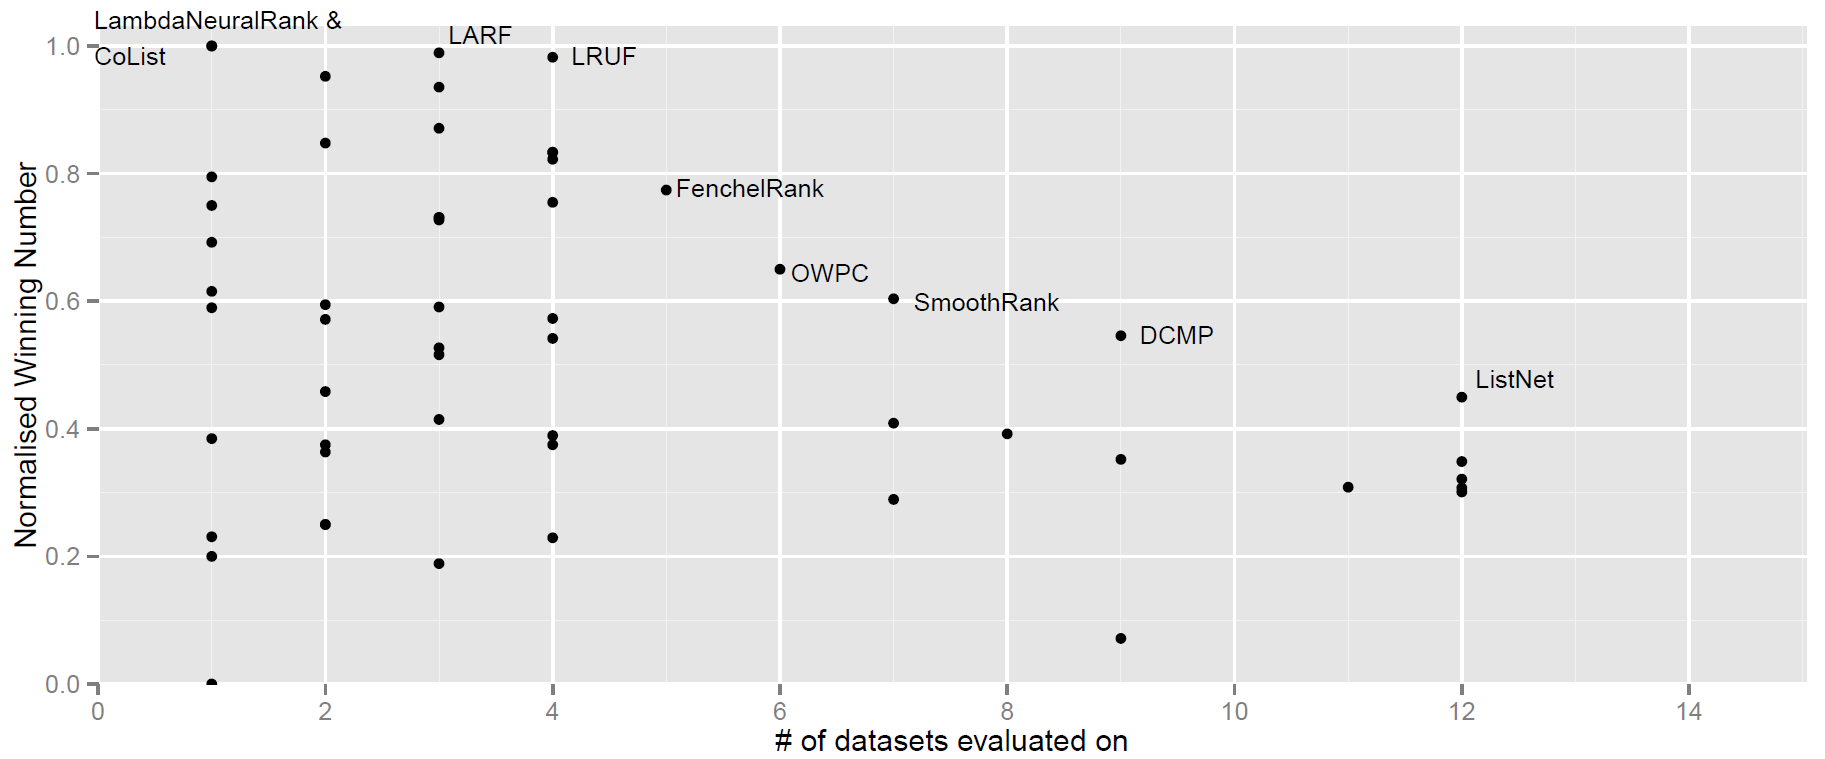
\includegraphics[scale=0.30]{gfx/ndcg3_winnum}
\caption{\acs{nDCG}@3 comparison of Learning-to-Rank methods}
\label{fig:normalised_winning_number_ndcg3}
\end{figure}

LambdaNeuralRank and CoList both acquired a perfect Normalised Winning Number score of 1.0 by beating all other algorithms on one dataset, with LambdaNeuralRank winning on the AOL dataset and CoList winning on Yahoo Set 2. LARF and LRUF both scored very high scores of near 1.0 on three of the LETOR 3.0 datasets, which can be said to have a higher degree of certainty on the methods' performance because they are validated on three datasets which in addition are more relevant datasets than AOL and Yahoo Set 2 because there are more evaluation results available for the LETOR 3.0 datasets. FenchelRank, OWPC, SmoothRank, DCMP and ListNet are in that order increasingly lower in Normalised Winning Number, but increasingly higher in number of datasets that they are evaluated on, resulting in a higher degree of certainty on the accuracy of the algorithms.\\

LambdaNeuralRank, CoList, LARF, LRUF, OWPC and DCMP evaluation results are all based on one study, therefore are subjected to the risk of one overly optimistic study producing those results. FenchelRank evaluation result are based combined result from two studies, although those studies have overlap in authors. SmoothRank and ListNet have the most reliable evaluation result source, as they were official LETOR baseline runs.  

\subsection{NDCG@5}
Figure \ref{fig:normalised_winning_number_ndcg5} shows the performance of Learning-to-Rank methods for the \ac{nDCG}@5 metric. Table \ref{tab:raw_data_norm_winnum_ndcg5} in Appendix \ref{app:norm_winnum_ndcg5} provides the raw Normalised Winning Number data for the Learning-to-Rank methods.\\

\begin{figure}[!h]
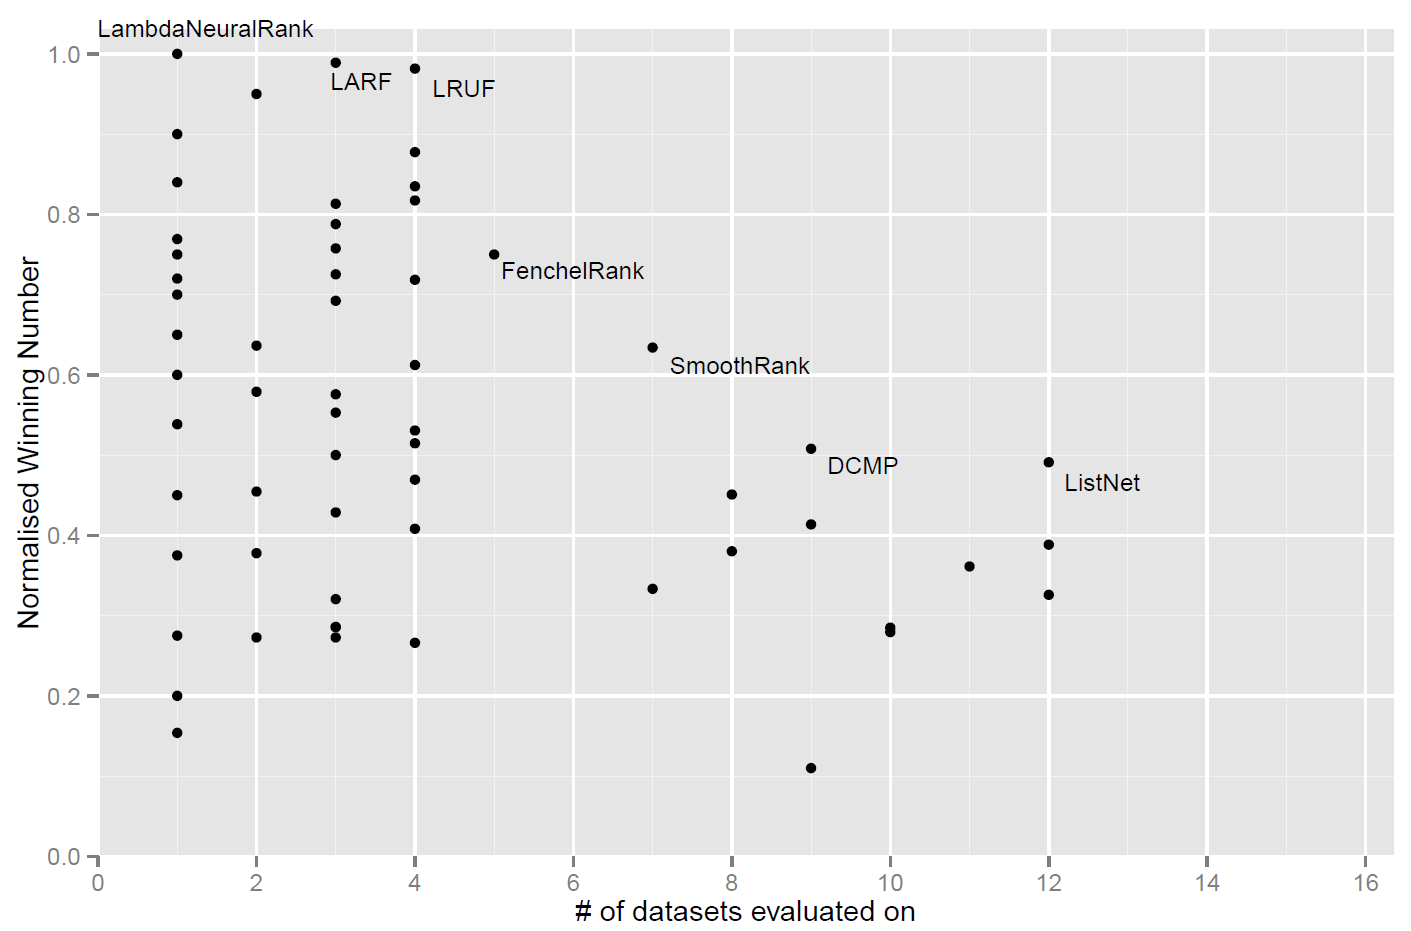
\includegraphics[scale=0.26]{gfx/ndcg5_winnum}
\caption{\acs{nDCG}@5 comparison of Learning-to-Rank methods}
\label{fig:normalised_winning_number_ndcg5}
\end{figure}

LambdaNeuralRank again beat all other methods solely with results on the AOL dataset scoring a Normalised Winning Number of 1.0. LARF, LRUF, FenchelRank, SmoothRank, DCMP and ListNet are from left to right evaluated on an increasing number of datasets, but score decreasingly well in terms of Normalised Winning Number. These results are highly in agreement with the \ac{nDCG}@3 comparison, with the only modification being that OWPC showed to be a method with no better method performing better on both axes in the \ac{nDCG}@3 comparison, but not in the \ac{nDCG}@5 comparison. Also in this comparison SmoothRank and ListNet can be regarded as most reliable results, as the evaluation measurements for these methods are based on LETOR official baselines.

\subsection{NDCG@10}
Figure \ref{fig:normalised_winning_number_ndcg10} shows the performance of Learning-to-Rank methods for the \ac{nDCG}@10 metric. Table \ref{tab:raw_data_norm_winnum_ndcg10} in Appendix \ref{app:norm_winnum_ndcg10} provides the raw Normalised Winning Number data for the Learning-to-Rank methods.\\

\begin{figure}[!h]
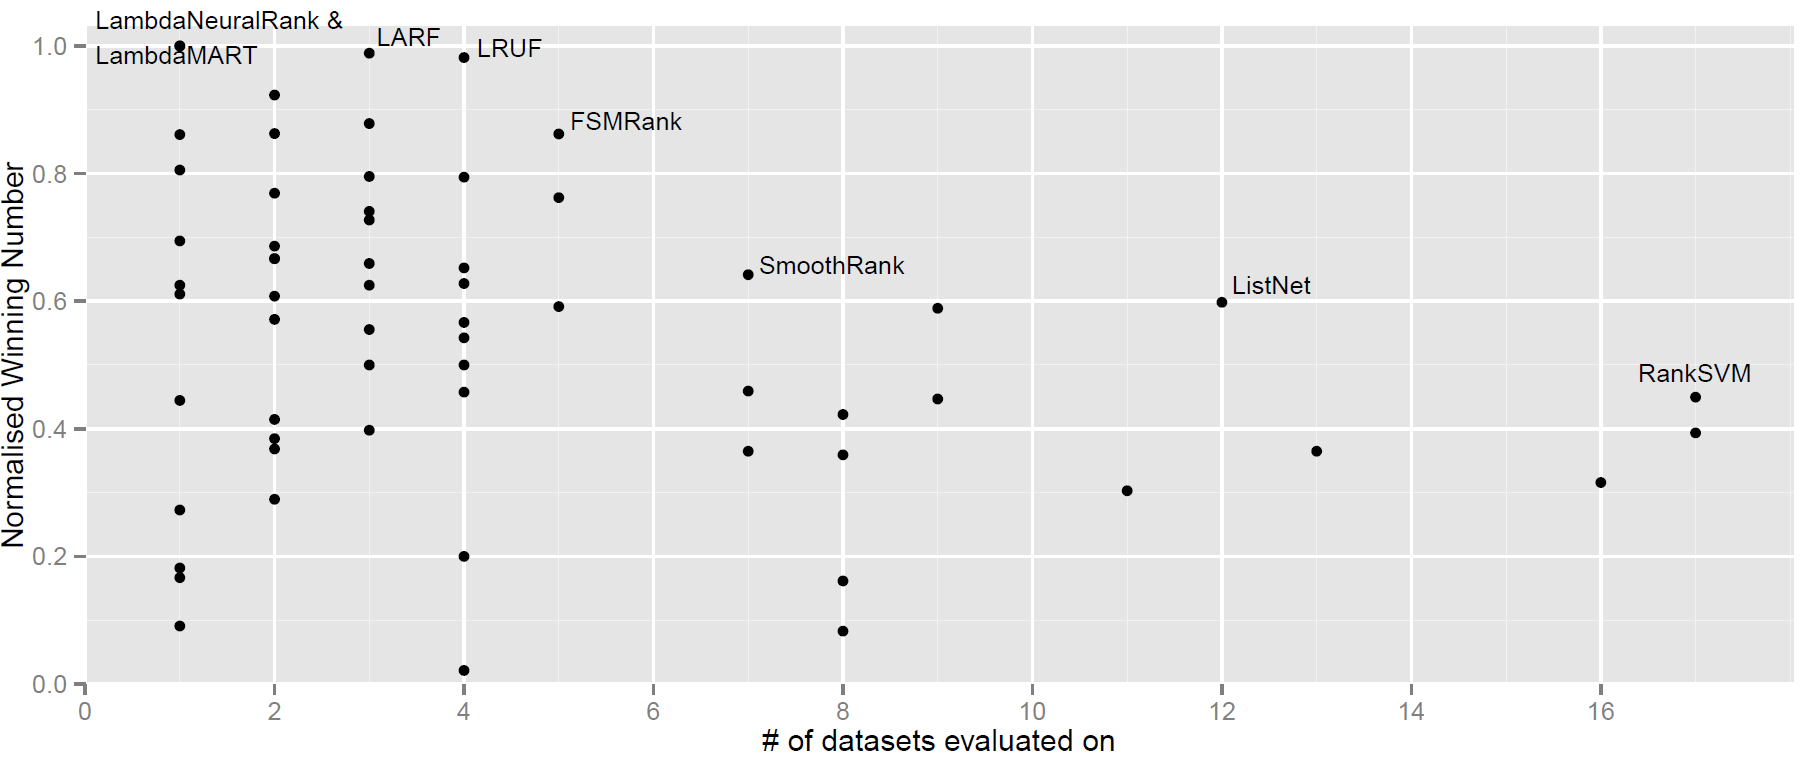
\includegraphics[scale=0.26]{gfx/ndcg10_winnum}
\caption{\acs{nDCG}@10 comparison of Learning-to-Rank methods}
\label{fig:normalised_winning_number_ndcg10}
\end{figure}

%TODO: Wat valt er te zeggen over de NDCG@10 resultaten? %

\subsection{MAP}
Figure \ref{fig:normalised_winning_number_map} shows the performance of Learning-to-Rank methods for the \ac{MAP} metric. Table \ref{tab:raw_data_norm_winnum_map} in Appendix \ref{app:norm_winnum_map} provides the raw Normalised Winning Number data for the Learning-to-Rank methods.\\

\begin{figure}[!h]
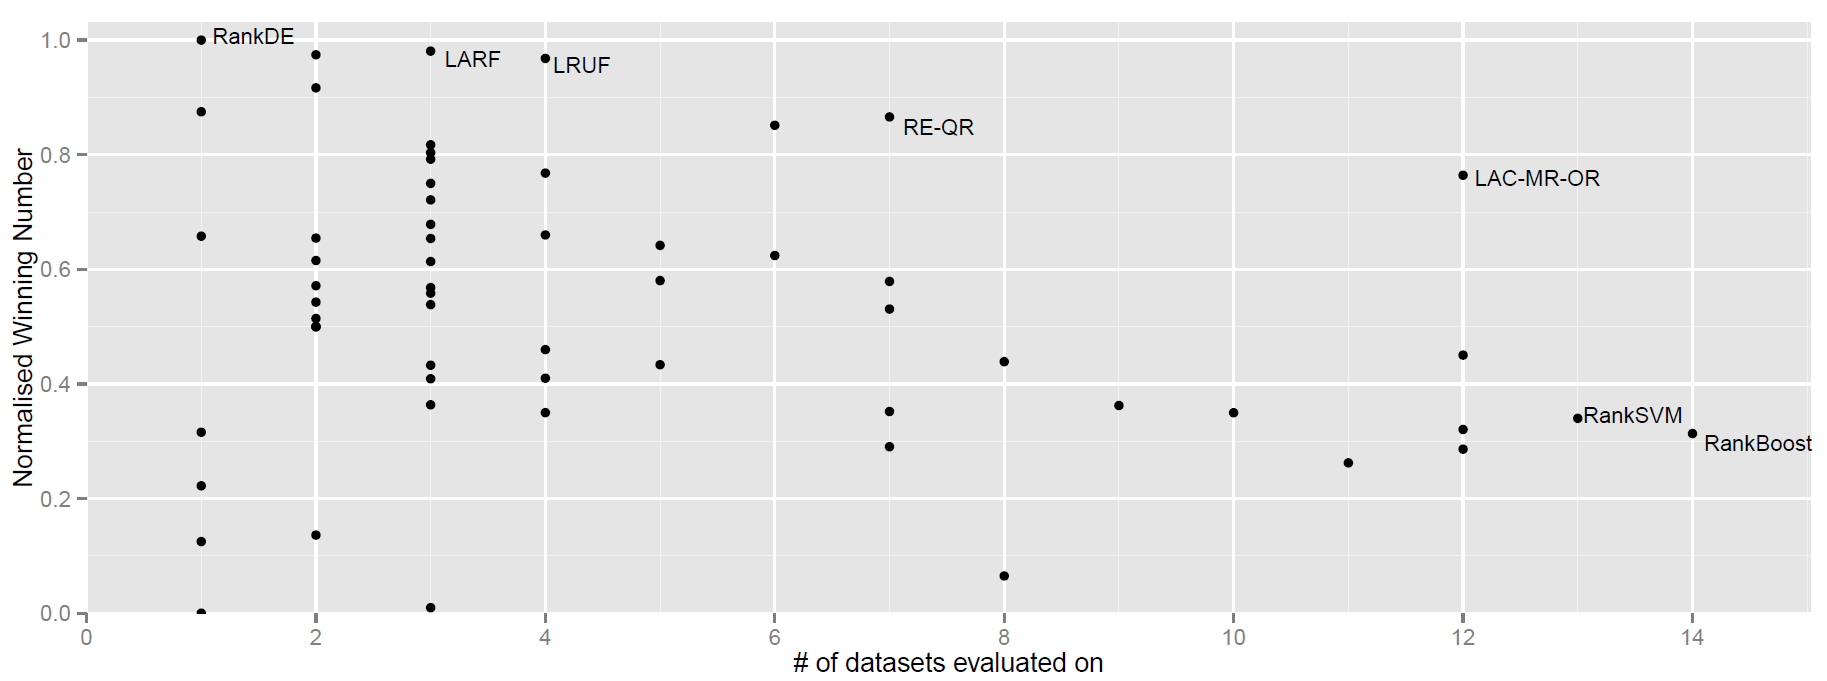
\includegraphics[scale=0.26]{gfx/map_winnum}
\caption{\acs{MAP} comparison of Learning-to-Rank methods}
\label{fig:normalised_winning_number_map}
\end{figure}

%TODO: Wat valt er te zeggen over de MAP resultaten? %

\subsection{Cross-metric}
Figure \ref{fig:normalised_winning_number_all} shows the Normalised Winning Number as function of Ideal Winning Number for the methods described in Table \ref{tab:ltr_methods_used}. Table \ref{tab:raw_data_norm_winnum_all} in Appendix \ref{app:norm_winnum_all} provide the raw data plotted in Figure \ref{fig:normalised_winning_number_all}.
\begin{figure}[!h]
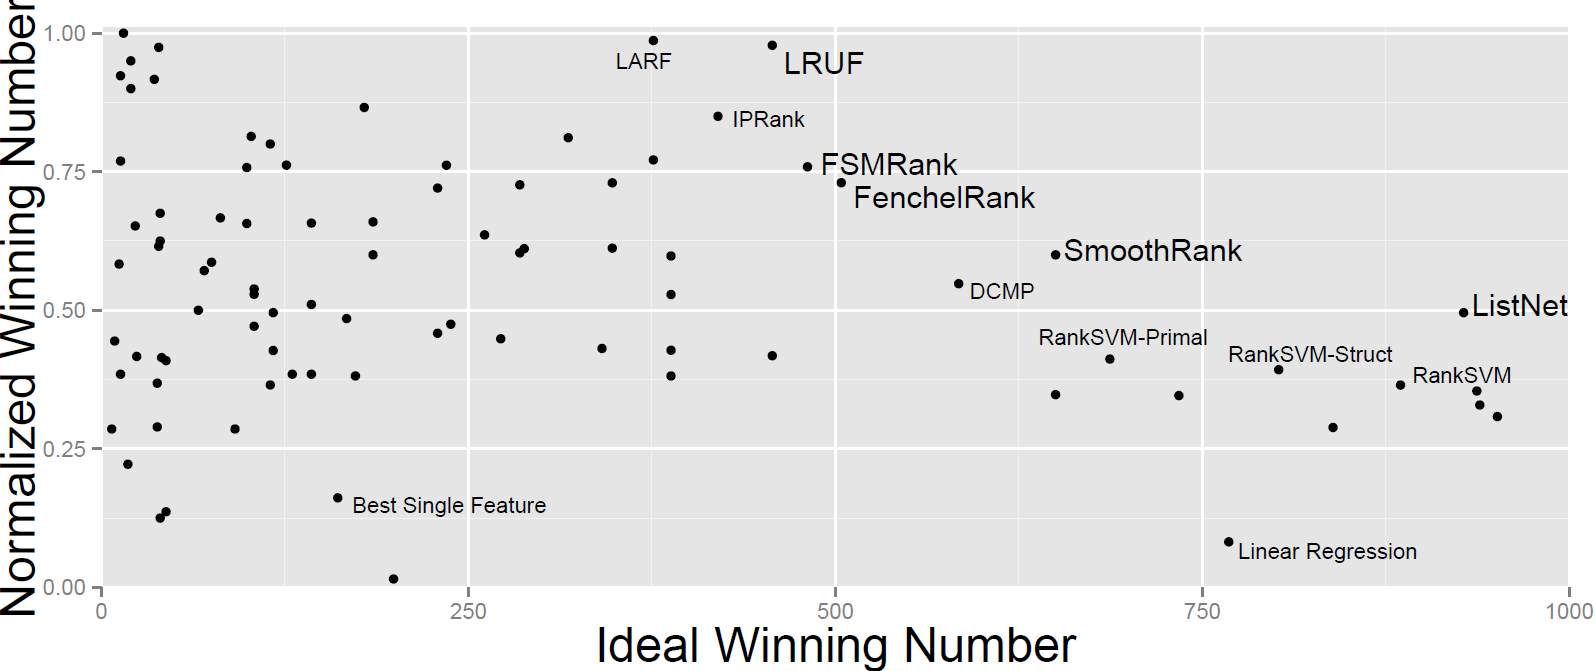
\includegraphics[scale=0.35]{gfx/combined_normalized_winnum}
\caption{Cross-benchmark comparison of Learning-to-Rank methods}
\label{fig:normalised_winning_number_all}
\end{figure}
%TODO: Wat valt er te zeggen over de cross-metric resultaten? %

\section{Limitations}
In the Normalised Winning Number calculation the weight of each benchmark on the total score is determined by the number of evaluation measurements on this benchmark. By calculating it in this way, we implicitly make the assumption that the Learning-to-Rank methods are (approximately) distributed uniformly over the benchmarks, such that the average Learning-to-Rank method tested are approximately equally hard for each data set. It could be the case however that this assumption is false and that one some datasets significantly better Learning-to-Rank methods are evaluated than on some other datasets.\\

A second limitation is that the datasets on which Learning-to-Rank methods have been evaluated can not always be regarded a random choice. It might be the case that some researchers chose to publish results for exactly those benchmark datasets that showed the most positive results for their Learning-to-Rank method.\\

Another limitation lies in the meta-analysis methodology. Using evaluation results published by other researchers relies on the honesty of those researchers. Overly optimistic evaluation results published by other researchers do affect our Normalised Winning Number results. Only including studies in the meta-analysis that comparable results on one of the baseline methods of a benchmark reduces this limitation but does not solve it. By taking the Ideal Winning Number into account in Figure \ref{fig:normalised_winning_number_all} we further mitigate this limitation, as the Ideal Winning Number is loosely related with the number of studies that reported evaluation results for an algorithm.

\section{Conclusions}